\documentclass[]{article}
\usepackage{lmodern}
\usepackage{amssymb,amsmath}
\usepackage{ifxetex,ifluatex}
\usepackage{fixltx2e} % provides \textsubscript
\ifnum 0\ifxetex 1\fi\ifluatex 1\fi=0 % if pdftex
  \usepackage[T1]{fontenc}
  \usepackage[utf8]{inputenc}
\else % if luatex or xelatex
  \ifxetex
    \usepackage{mathspec}
  \else
    \usepackage{fontspec}
  \fi
  \defaultfontfeatures{Ligatures=TeX,Scale=MatchLowercase}
\fi
% use upquote if available, for straight quotes in verbatim environments
\IfFileExists{upquote.sty}{\usepackage{upquote}}{}
% use microtype if available
\IfFileExists{microtype.sty}{%
\usepackage{microtype}
\UseMicrotypeSet[protrusion]{basicmath} % disable protrusion for tt fonts
}{}
\usepackage[margin=1in]{geometry}
\usepackage{hyperref}
\hypersetup{unicode=true,
            pdftitle={Project},
            pdfauthor={Matthew Fein},
            pdfborder={0 0 0},
            breaklinks=true}
\urlstyle{same}  % don't use monospace font for urls
\usepackage{color}
\usepackage{fancyvrb}
\newcommand{\VerbBar}{|}
\newcommand{\VERB}{\Verb[commandchars=\\\{\}]}
\DefineVerbatimEnvironment{Highlighting}{Verbatim}{commandchars=\\\{\}}
% Add ',fontsize=\small' for more characters per line
\usepackage{framed}
\definecolor{shadecolor}{RGB}{248,248,248}
\newenvironment{Shaded}{\begin{snugshade}}{\end{snugshade}}
\newcommand{\KeywordTok}[1]{\textcolor[rgb]{0.13,0.29,0.53}{\textbf{#1}}}
\newcommand{\DataTypeTok}[1]{\textcolor[rgb]{0.13,0.29,0.53}{#1}}
\newcommand{\DecValTok}[1]{\textcolor[rgb]{0.00,0.00,0.81}{#1}}
\newcommand{\BaseNTok}[1]{\textcolor[rgb]{0.00,0.00,0.81}{#1}}
\newcommand{\FloatTok}[1]{\textcolor[rgb]{0.00,0.00,0.81}{#1}}
\newcommand{\ConstantTok}[1]{\textcolor[rgb]{0.00,0.00,0.00}{#1}}
\newcommand{\CharTok}[1]{\textcolor[rgb]{0.31,0.60,0.02}{#1}}
\newcommand{\SpecialCharTok}[1]{\textcolor[rgb]{0.00,0.00,0.00}{#1}}
\newcommand{\StringTok}[1]{\textcolor[rgb]{0.31,0.60,0.02}{#1}}
\newcommand{\VerbatimStringTok}[1]{\textcolor[rgb]{0.31,0.60,0.02}{#1}}
\newcommand{\SpecialStringTok}[1]{\textcolor[rgb]{0.31,0.60,0.02}{#1}}
\newcommand{\ImportTok}[1]{#1}
\newcommand{\CommentTok}[1]{\textcolor[rgb]{0.56,0.35,0.01}{\textit{#1}}}
\newcommand{\DocumentationTok}[1]{\textcolor[rgb]{0.56,0.35,0.01}{\textbf{\textit{#1}}}}
\newcommand{\AnnotationTok}[1]{\textcolor[rgb]{0.56,0.35,0.01}{\textbf{\textit{#1}}}}
\newcommand{\CommentVarTok}[1]{\textcolor[rgb]{0.56,0.35,0.01}{\textbf{\textit{#1}}}}
\newcommand{\OtherTok}[1]{\textcolor[rgb]{0.56,0.35,0.01}{#1}}
\newcommand{\FunctionTok}[1]{\textcolor[rgb]{0.00,0.00,0.00}{#1}}
\newcommand{\VariableTok}[1]{\textcolor[rgb]{0.00,0.00,0.00}{#1}}
\newcommand{\ControlFlowTok}[1]{\textcolor[rgb]{0.13,0.29,0.53}{\textbf{#1}}}
\newcommand{\OperatorTok}[1]{\textcolor[rgb]{0.81,0.36,0.00}{\textbf{#1}}}
\newcommand{\BuiltInTok}[1]{#1}
\newcommand{\ExtensionTok}[1]{#1}
\newcommand{\PreprocessorTok}[1]{\textcolor[rgb]{0.56,0.35,0.01}{\textit{#1}}}
\newcommand{\AttributeTok}[1]{\textcolor[rgb]{0.77,0.63,0.00}{#1}}
\newcommand{\RegionMarkerTok}[1]{#1}
\newcommand{\InformationTok}[1]{\textcolor[rgb]{0.56,0.35,0.01}{\textbf{\textit{#1}}}}
\newcommand{\WarningTok}[1]{\textcolor[rgb]{0.56,0.35,0.01}{\textbf{\textit{#1}}}}
\newcommand{\AlertTok}[1]{\textcolor[rgb]{0.94,0.16,0.16}{#1}}
\newcommand{\ErrorTok}[1]{\textcolor[rgb]{0.64,0.00,0.00}{\textbf{#1}}}
\newcommand{\NormalTok}[1]{#1}
\usepackage{graphicx,grffile}
\makeatletter
\def\maxwidth{\ifdim\Gin@nat@width>\linewidth\linewidth\else\Gin@nat@width\fi}
\def\maxheight{\ifdim\Gin@nat@height>\textheight\textheight\else\Gin@nat@height\fi}
\makeatother
% Scale images if necessary, so that they will not overflow the page
% margins by default, and it is still possible to overwrite the defaults
% using explicit options in \includegraphics[width, height, ...]{}
\setkeys{Gin}{width=\maxwidth,height=\maxheight,keepaspectratio}
\IfFileExists{parskip.sty}{%
\usepackage{parskip}
}{% else
\setlength{\parindent}{0pt}
\setlength{\parskip}{6pt plus 2pt minus 1pt}
}
\setlength{\emergencystretch}{3em}  % prevent overfull lines
\providecommand{\tightlist}{%
  \setlength{\itemsep}{0pt}\setlength{\parskip}{0pt}}
\setcounter{secnumdepth}{0}
% Redefines (sub)paragraphs to behave more like sections
\ifx\paragraph\undefined\else
\let\oldparagraph\paragraph
\renewcommand{\paragraph}[1]{\oldparagraph{#1}\mbox{}}
\fi
\ifx\subparagraph\undefined\else
\let\oldsubparagraph\subparagraph
\renewcommand{\subparagraph}[1]{\oldsubparagraph{#1}\mbox{}}
\fi

%%% Use protect on footnotes to avoid problems with footnotes in titles
\let\rmarkdownfootnote\footnote%
\def\footnote{\protect\rmarkdownfootnote}

%%% Change title format to be more compact
\usepackage{titling}

% Create subtitle command for use in maketitle
\newcommand{\subtitle}[1]{
  \posttitle{
    \begin{center}\large#1\end{center}
    }
}

\setlength{\droptitle}{-2em}

  \title{Project}
    \pretitle{\vspace{\droptitle}\centering\huge}
  \posttitle{\par}
    \author{Matthew Fein}
    \preauthor{\centering\large\emph}
  \postauthor{\par}
      \predate{\centering\large\emph}
  \postdate{\par}
    \date{April 15, 2019}


\begin{document}
\maketitle

\subsection{Machine Learning Final Project- telecom churn
data}\label{machine-learning-final-project--telecom-churn-data}

\begin{Shaded}
\begin{Highlighting}[]
\KeywordTok{require}\NormalTok{(tidyverse)}
\end{Highlighting}
\end{Shaded}

\begin{verbatim}
## Loading required package: tidyverse
\end{verbatim}

\begin{verbatim}
## -- Attaching packages -------------------------------------- tidyverse 1.2.1 --
\end{verbatim}

\begin{verbatim}
## v ggplot2 3.0.0     v purrr   0.2.5
## v tibble  1.4.2     v dplyr   0.7.6
## v tidyr   0.8.1     v stringr 1.3.1
## v readr   1.1.1     v forcats 0.3.0
\end{verbatim}

\begin{verbatim}
## -- Conflicts ----------------------------------------- tidyverse_conflicts() --
## x dplyr::filter() masks stats::filter()
## x dplyr::lag()    masks stats::lag()
\end{verbatim}

\begin{Shaded}
\begin{Highlighting}[]
\KeywordTok{require}\NormalTok{(glmnet)}
\end{Highlighting}
\end{Shaded}

\begin{verbatim}
## Loading required package: glmnet
\end{verbatim}

\begin{verbatim}
## Warning: package 'glmnet' was built under R version 3.5.2
\end{verbatim}

\begin{verbatim}
## Loading required package: Matrix
\end{verbatim}

\begin{verbatim}
## 
## Attaching package: 'Matrix'
\end{verbatim}

\begin{verbatim}
## The following object is masked from 'package:tidyr':
## 
##     expand
\end{verbatim}

\begin{verbatim}
## Loading required package: foreach
\end{verbatim}

\begin{verbatim}
## Warning: package 'foreach' was built under R version 3.5.2
\end{verbatim}

\begin{verbatim}
## 
## Attaching package: 'foreach'
\end{verbatim}

\begin{verbatim}
## The following objects are masked from 'package:purrr':
## 
##     accumulate, when
\end{verbatim}

\begin{verbatim}
## Loaded glmnet 2.0-16
\end{verbatim}

\begin{Shaded}
\begin{Highlighting}[]
\KeywordTok{require}\NormalTok{(ISLR)}
\end{Highlighting}
\end{Shaded}

\begin{verbatim}
## Loading required package: ISLR
\end{verbatim}

\begin{verbatim}
## Warning: package 'ISLR' was built under R version 3.5.2
\end{verbatim}

\begin{Shaded}
\begin{Highlighting}[]
\KeywordTok{require}\NormalTok{(MASS)}
\end{Highlighting}
\end{Shaded}

\begin{verbatim}
## Loading required package: MASS
\end{verbatim}

\begin{verbatim}
## 
## Attaching package: 'MASS'
\end{verbatim}

\begin{verbatim}
## The following object is masked from 'package:dplyr':
## 
##     select
\end{verbatim}

\begin{Shaded}
\begin{Highlighting}[]
\CommentTok{# Import data with strings as factors}
\NormalTok{data.all <-}\StringTok{ }\KeywordTok{read.csv}\NormalTok{(}\StringTok{"bigml_59c28831336c6604c800002a.csv"}\NormalTok{)}
\CommentTok{#clean data for analysis by removing uninformative attributes (phone number and state)}
\NormalTok{data.cl <-}\StringTok{ }\NormalTok{data.all[ , }\OperatorTok{-}\KeywordTok{c}\NormalTok{(}\DecValTok{1}\OperatorTok{:}\DecValTok{4}\NormalTok{)]}
\end{Highlighting}
\end{Shaded}

\subsection{EDA looking at correlation
matrices}\label{eda-looking-at-correlation-matrices}

\begin{Shaded}
\begin{Highlighting}[]
\CommentTok{#uninterpretable}
\KeywordTok{pairs}\NormalTok{(data.cl, }\DataTypeTok{col=}\NormalTok{ data.cl}\OperatorTok{$}\NormalTok{churn)}
\end{Highlighting}
\end{Shaded}

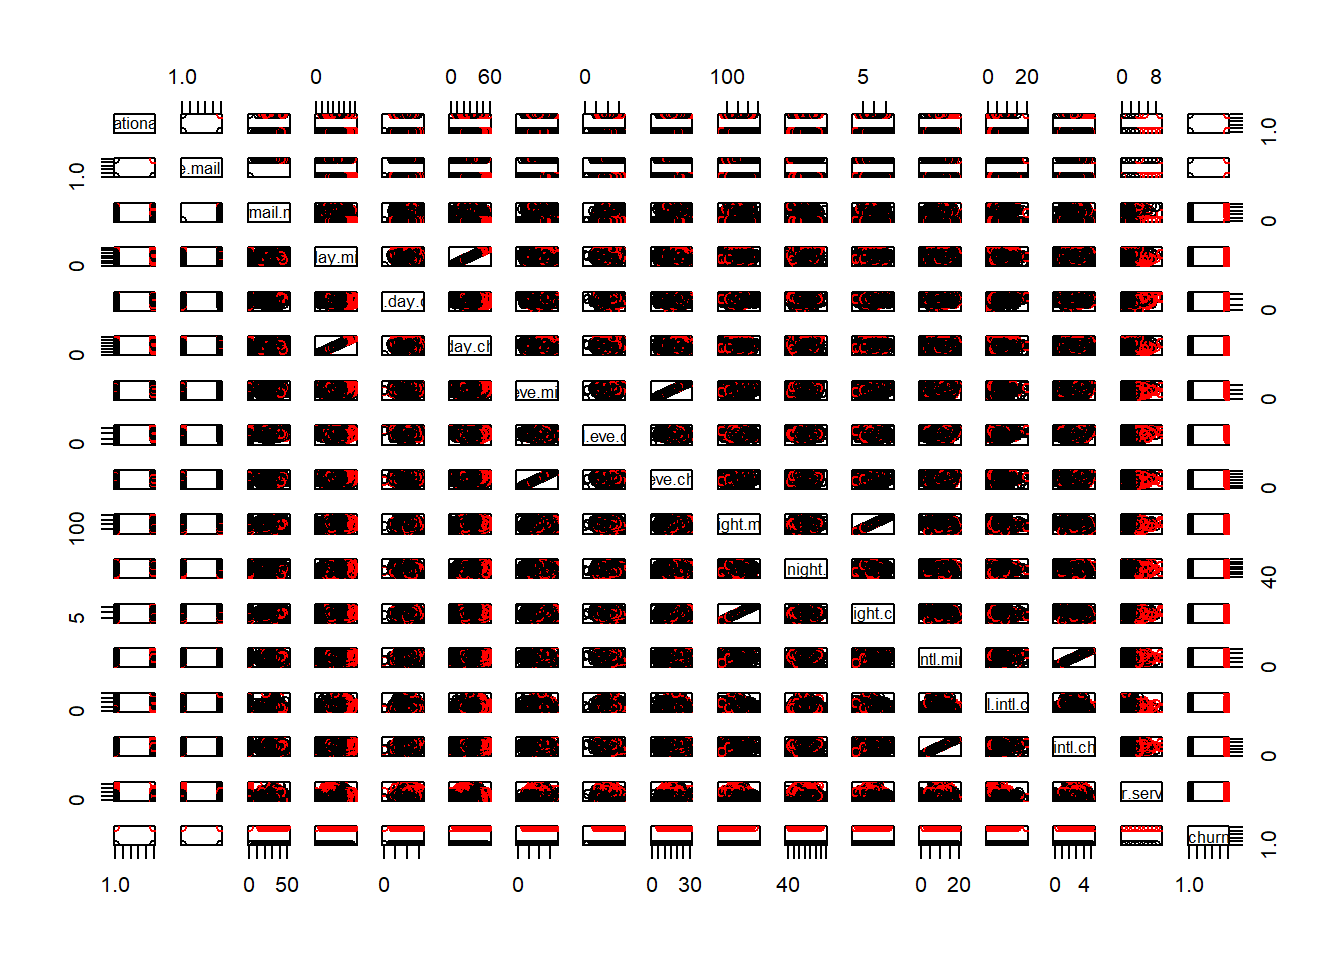
\includegraphics{churn_files/figure-latex/eda-1.pdf}

\begin{Shaded}
\begin{Highlighting}[]
\CommentTok{#zoom in}
\KeywordTok{pairs}\NormalTok{(data.cl[ , }\OperatorTok{-}\StringTok{ }\KeywordTok{c}\NormalTok{(}\DecValTok{1}\OperatorTok{:}\DecValTok{2}\NormalTok{,}\DecValTok{17}\NormalTok{)], }\DataTypeTok{col =}\NormalTok{ data.cl}\OperatorTok{$}\NormalTok{churn)}
\end{Highlighting}
\end{Shaded}

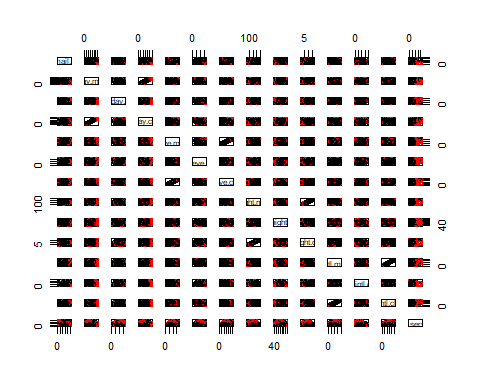
\includegraphics{churn_files/figure-latex/eda-2.pdf}

\begin{Shaded}
\begin{Highlighting}[]
\CommentTok{#High multicollinearity between minutes and charges- removed minutes and kept charges}
\NormalTok{data.cl <-}\StringTok{ }\NormalTok{data.cl[ , }\OperatorTok{-}\KeywordTok{c}\NormalTok{(}\DecValTok{4}\NormalTok{,}\DecValTok{7}\NormalTok{,}\DecValTok{10}\NormalTok{,}\DecValTok{13}\NormalTok{)]}
\end{Highlighting}
\end{Shaded}

Partition data

\begin{Shaded}
\begin{Highlighting}[]
\NormalTok{train <-}\StringTok{ }\NormalTok{data.cl[}\DecValTok{1}\OperatorTok{:}\DecValTok{2222}\NormalTok{, ]}
\NormalTok{test <-}\StringTok{ }\NormalTok{data.cl[}\DecValTok{2223}\OperatorTok{:}\DecValTok{3333}\NormalTok{, ]}
\end{Highlighting}
\end{Shaded}

Utilize LASSO for feature selection

\begin{Shaded}
\begin{Highlighting}[]
\NormalTok{lasso.x =}\StringTok{ }\KeywordTok{model.matrix}\NormalTok{(}\KeywordTok{glm}\NormalTok{(churn}\OperatorTok{~}\NormalTok{.}\OperatorTok{-}\NormalTok{churn, }\DataTypeTok{data =}\NormalTok{ train, }\DataTypeTok{family =}\NormalTok{ binomial))[,}\OperatorTok{-}\DecValTok{1}\NormalTok{]}
\NormalTok{lasso.x2 =}\StringTok{ }\KeywordTok{model.matrix}\NormalTok{(}\KeywordTok{glm}\NormalTok{(churn}\OperatorTok{~}\NormalTok{.}\OperatorTok{-}\NormalTok{churn, }\DataTypeTok{data =}\NormalTok{ test, }\DataTypeTok{family =}\NormalTok{ binomial))[,}\OperatorTok{-}\DecValTok{1}\NormalTok{]}
\NormalTok{y.train =}\StringTok{ }\KeywordTok{as.integer}\NormalTok{(train}\OperatorTok{$}\NormalTok{churn)}
\NormalTok{y.test <-}\StringTok{ }\KeywordTok{as.integer}\NormalTok{(test}\OperatorTok{$}\NormalTok{churn)}

\NormalTok{lasso.mod=}\KeywordTok{glmnet}\NormalTok{(lasso.x,y.train,}\DataTypeTok{alpha=}\DecValTok{1}\NormalTok{)}
\KeywordTok{plot}\NormalTok{(lasso.mod)}
\end{Highlighting}
\end{Shaded}

\includegraphics{churn_files/figure-latex/unnamed-chunk-3-1.pdf}

\begin{Shaded}
\begin{Highlighting}[]
\NormalTok{cv.out=}\KeywordTok{cv.glmnet}\NormalTok{(lasso.x,y.train,}\DataTypeTok{alpha=}\DecValTok{1}\NormalTok{)}
\KeywordTok{plot}\NormalTok{(cv.out)}
\end{Highlighting}
\end{Shaded}

\includegraphics{churn_files/figure-latex/unnamed-chunk-3-2.pdf}

\begin{Shaded}
\begin{Highlighting}[]
\NormalTok{bestlam=cv.out}\OperatorTok{$}\NormalTok{lambda.min}
\NormalTok{lasso.pred=}\KeywordTok{predict}\NormalTok{(lasso.mod,}\DataTypeTok{s=}\NormalTok{bestlam,}\DataTypeTok{newx=}\NormalTok{lasso.x2)}
\KeywordTok{mean}\NormalTok{((lasso.pred}\OperatorTok{-}\NormalTok{y.test)}\OperatorTok{^}\DecValTok{2}\NormalTok{)}
\end{Highlighting}
\end{Shaded}

\begin{verbatim}
## [1] 0.1095457
\end{verbatim}

\begin{Shaded}
\begin{Highlighting}[]
\NormalTok{out=}\KeywordTok{glmnet}\NormalTok{(lasso.x,y.train,}\DataTypeTok{alpha=}\DecValTok{1}\NormalTok{)}
\NormalTok{lasso.coef=}\KeywordTok{predict}\NormalTok{(out,}\DataTypeTok{type=}\StringTok{"coefficients"}\NormalTok{,}\DataTypeTok{s=}\NormalTok{bestlam)}
\NormalTok{lasso.coef}
\end{Highlighting}
\end{Shaded}

\begin{verbatim}
## 13 x 1 sparse Matrix of class "dgCMatrix"
##                                    1
## (Intercept)             6.150076e-01
## international.planyes   2.869477e-01
## voice.mail.planyes     -7.207318e-02
## number.vmail.messages   .           
## total.day.calls         4.127394e-05
## total.day.charge        6.318496e-03
## total.eve.calls         .           
## total.eve.charge        6.389826e-03
## total.night.calls      -3.293795e-05
## total.night.charge      7.424842e-03
## total.intl.calls       -3.968562e-03
## total.intl.charge       2.996543e-02
## customer.service.calls  5.089376e-02
\end{verbatim}

\begin{Shaded}
\begin{Highlighting}[]
\NormalTok{lasso.coef[lasso.coef}\OperatorTok{!=}\DecValTok{0}\NormalTok{]}
\end{Highlighting}
\end{Shaded}

\begin{verbatim}
## <sparse>[ <logic> ] : .M.sub.i.logical() maybe inefficient
\end{verbatim}

\begin{verbatim}
##  [1]  6.150076e-01  2.869477e-01 -7.207318e-02  4.127394e-05  6.318496e-03
##  [6]  6.389826e-03 -3.293795e-05  7.424842e-03 -3.968562e-03  2.996543e-02
## [11]  5.089376e-02
\end{verbatim}


\end{document}
